\section{Dirichlet Condition Coarsening}
To coarsening Dirichlet conditions, we choice the geometric coarsening strategy introduced in Section~\ref{sec:geo_coarsen}, with some modifications. Dirichlet condition are imposed at cell granularity. At top level Dirichlet cells are marked \textit{X Dirichlet}, \textit{Y Dirichlet}, \textit{Z Dirichlet}, or any combination of the three based on which degrees of freedom are fixed. If a cell is marked Dirichlet, all of its nodes are marked Dirichlet as well. 

For the coarse level, the additional rotational degrees of freedom also needs to be marked as Dirichlet. For 2D, if a cell is fixed, either in X or Y, it will not be able to rotate, therefore the rotational degrees of freedom at the coarse level will also be marked as Dirichlet. For 3D, if a cell is fixed in X dimension, the cell would not be able to rotate in Y and Z axis, but still allows to rotate in X axis. Therefore, in this case, only the rotational degrees of freedom associated with Y axis rotation and Z axis rotation are marked as Dirichlet, the X axis rotation remains free.

\section{Choice of Smoother}
In Section~\ref{sec:Prolongation_Coarse}, a defect of the method was noted, that the coarse level,  $\hat{\epsilon}_1$ may not be $\in \text{Range}(\mathbf{L}^{(p)}_{ff})$ for Theorem~\ref{theo:p_solution}. This implies that for some nodes, the local convergence metric can be $K_{i,p} = \infty$. In such cases, a point based smoother may not sufficient. Therefore, for all the coarse levels, a colored box smoother of radius $2$ is used. This problem does not exist at the finest level, therefore, an eight-colored Guass-Seidel smoother is used at the finest level as presented in Section~\ref{sec:topopt_multigrid}. 

Because of that our Dirichlet condition is geometrically coarsened, to ensure the multigrid is stable, we will need extra boundary smoothing iterations. The boundary nodes are defined as: within $\mathbf{3}$ stencil distance from a Dirichlet node. For box smoother, we use boundary cells, defined as: within $\mathbf{2}$ cell radius in either axis of a Dirichlet cell. When using this stencil aware multigrid scheme as a preconditioner for conjugate gradient, we found a standard 3-1-3 scheme: 3 boundary smoothing, 1 interior smoothing, and 3 boundary smoothing again, is sufficient. In practice, we found that for boundary smoothing, Gauss-Seidel smoother is sufficient. While for interior smoothing, box smoother is needed for better convergence.

\section{Stencil Aware Multigrid as Preconditioner}
For better convergence behavior, instead of using the stencil aware multigrid as a standalone solver, we used a symmetric implementation of it to use it as a preconditioner for conjugate gradient.

For better convergence and avoiding null space in local problem, we also choice to pad the domain at the finest level with cells with minimal stiffness (1e-9) , but only for the preconditioner. So that all finest cells contained within the coarse cells at the lowest level has a valid stiffness. 
 \section{Solver Convergence Analysis}
 To test the solver convergence in comparison to standard multilinear interpolated multigrid, we conducted tests both synthetic and naturally emerged from topology optimization process.
 \subsection{Two Level Convergence Test}
  \begin{figure}[t]
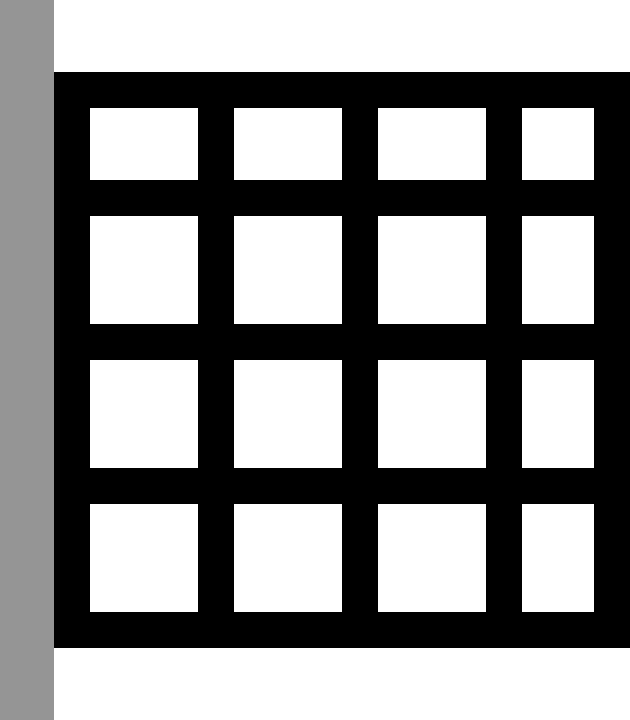
\includegraphics[width=5cm]{BBMG/synthetic_domain.png}
\centering
\caption{An illustration of the synthetic testing domain of $32^2$ in 2D. The left side is fixed as Dirichlet condition. Black region are solid materials, the white space in between are soft material of $10^{-9}$ stiffness. Material properties are: $\mu = 100$ and $\lambda = 200$. A uniform downward force is applied to the right face.}
\label{fig:synthetic_domain}
\end{figure}
 The two level convergence test is conducted on a synthetic domain of size $32^3$, Figure~\ref{fig:synthetic_domain}. Figure~\ref{fig:Two_Level_Convergence} shows the convergence rate of different methods for the synthetic domain. We can see that multi-linear multigrid (MLMG), convergence rate has drastically slowed down after 10 iterations, while stencil aware multigrid (SAMG) maintained the convergence rate of 0.5, that the residual reduces by half every iteration. Using stencil aware multigrid as a preconditioner for conjugate gradient (SAMGPCG), can even further improves convergence rate.
   \begin{figure}[t]
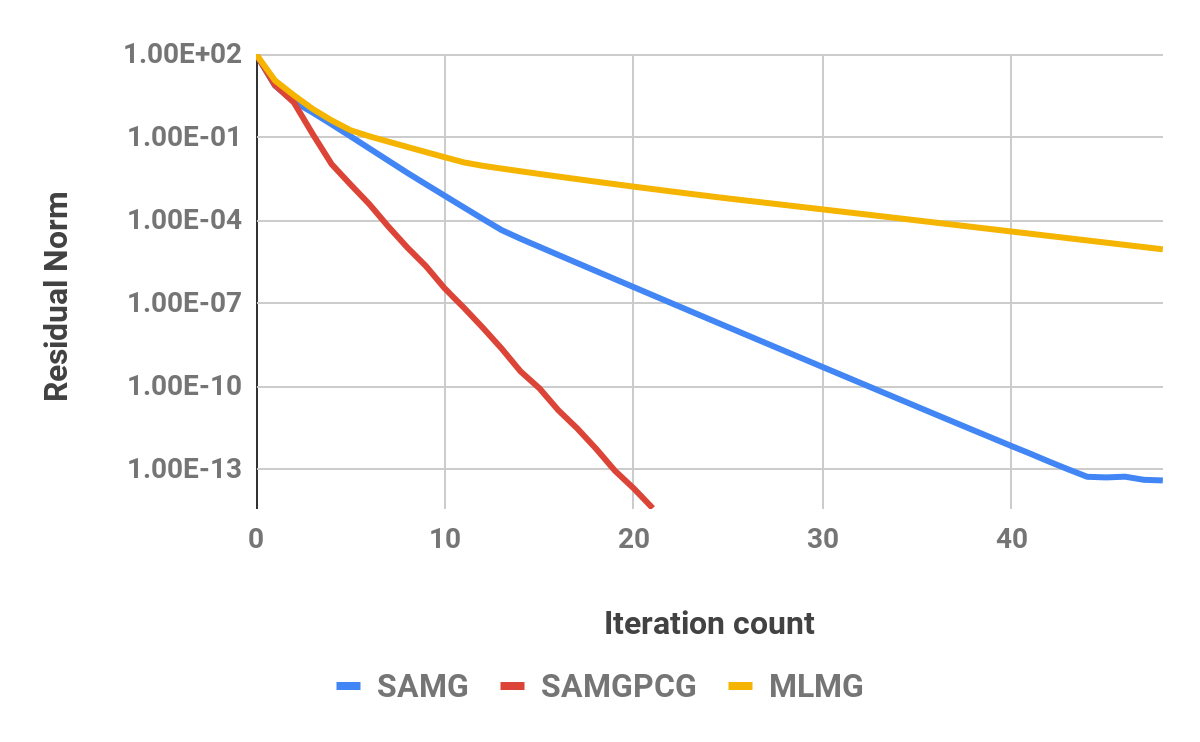
\includegraphics[width=10cm]{BBMG/Two_Level_Convergence.png}
\centering
\caption{Two level convergence rate of multilinear multigrid(MLMG), stencil aware multigrid(SAMG), and stencil aware multigrid preconditioned conjugate gradient(SAMGPCG) on the $32^3$ synthetic domain.}
\label{fig:Two_Level_Convergence}
\end{figure}
 \subsection{Multi-level Convergence Test}
 The convergence tests conducted were aimed to support the following hypothesis:
 \begin{enumerate}
 \item The convergence rate of \textit{multi-linear multigrid (MLMG)} preconditioned conjugate gradient combined with a \textit{colored Gauss-Seidel smoother}, slows down with the increasing resolution as more complex topology emerges.
  \item The convergence rate of \textit{multi-linear multigrid (MLMG)} preconditioned conjugate gradient combined with a \textit{colored box smoother}, slows down with the increasing resolution as more complex topology emerges.
 \item The convergence rate of \textit{stencil aware multigrid (SAMG)} preconditioned conjugate gradient combining with a  \textit{colored Gauss-Seidel smoother}, slows down with the increasing resolution as more complex topology emerges.
 \item The convergence rate of \textit{stencil aware multigrid (SAMG)} preconditioned conjugate gradient combining with a \textit{colored box smoother} is more consistent across different resolutions.
 \end{enumerate}
  The test is conducted using the bird beak topology optimization example, Figure~\ref{fig:beak}, at resolution $500 \times 400 \times 300$, $750 \times 600 \times 450$, and $1000 \times 800 \times 600$. The numbers of active voxels are 5M, 14M, and 40M. The last iteration of topology optimization is used.
 \subsubsection{Resolution Scale Test}
 Figure~\ref{fig:Bird_Beak_Convergence_Test}, top left plot, illustrates is the convergence rate of the MLMGPCG proposed in Chapter~\ref{Chapter:Elasticity}. The convergence rate of the algorithm decays with the increasing of the resolution. For 5M active voxels, the algorithm takes 120 iterations to reduce the initial residual by 5 orders of magnitude. While with 40M active voxels, it takes about 200 iterations to reduce the initial residual by 5 orders of magnitude.
 
Figure~\ref{fig:Bird_Beak_Convergence_Test}, top right plot, shows that by using a box smoother, the total number of iterations for convergence has reduced by 30\%. But with increment of resolution, we still observes a slow down in convergence.

Figure~\ref{fig:Bird_Beak_Convergence_Test}, bottom left plot, shows that by using a box smoother, the total number of iterations for convergence has reduced by 30\%. But with increment of resolution, we still observes a slow down in convergence.
 \begin{figure}[t]
 \begin{subfigure}[t]{0.5\textwidth}
 \centering
 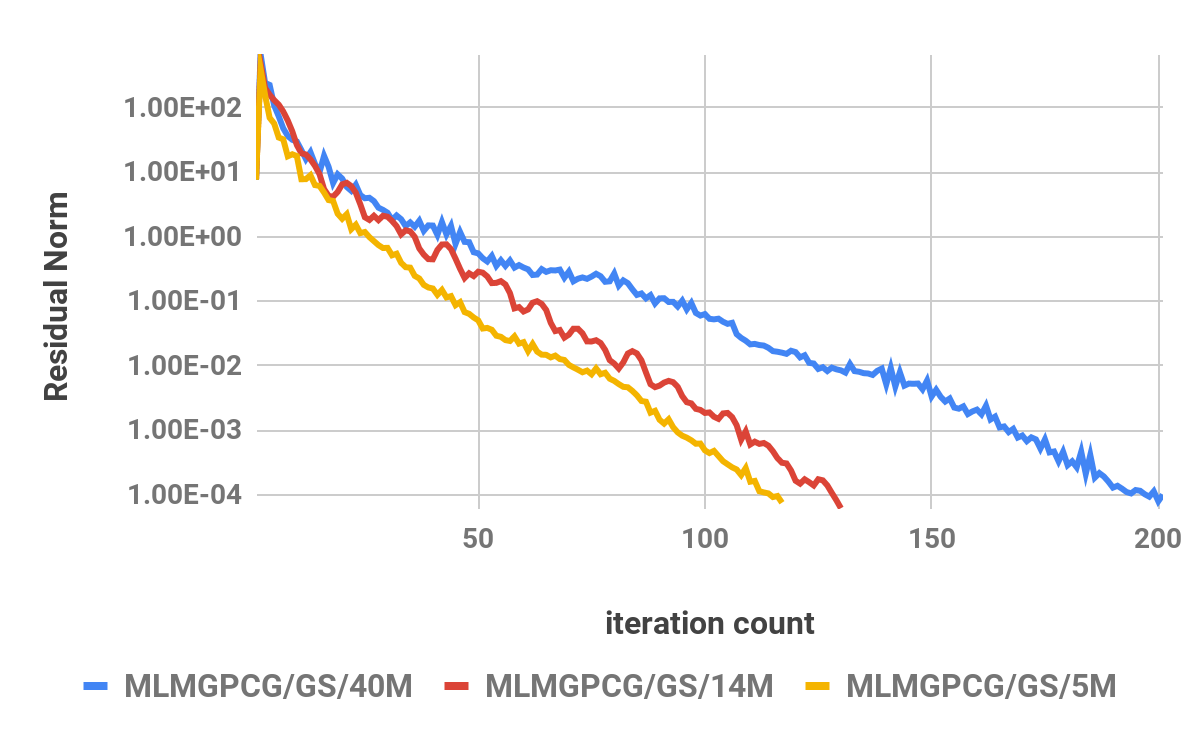
\includegraphics[width=\textwidth]{BBMG/MLMGPCG_GS.png}
 \end{subfigure}
 \begin{subfigure}[t]{0.5\textwidth}
 \centering
 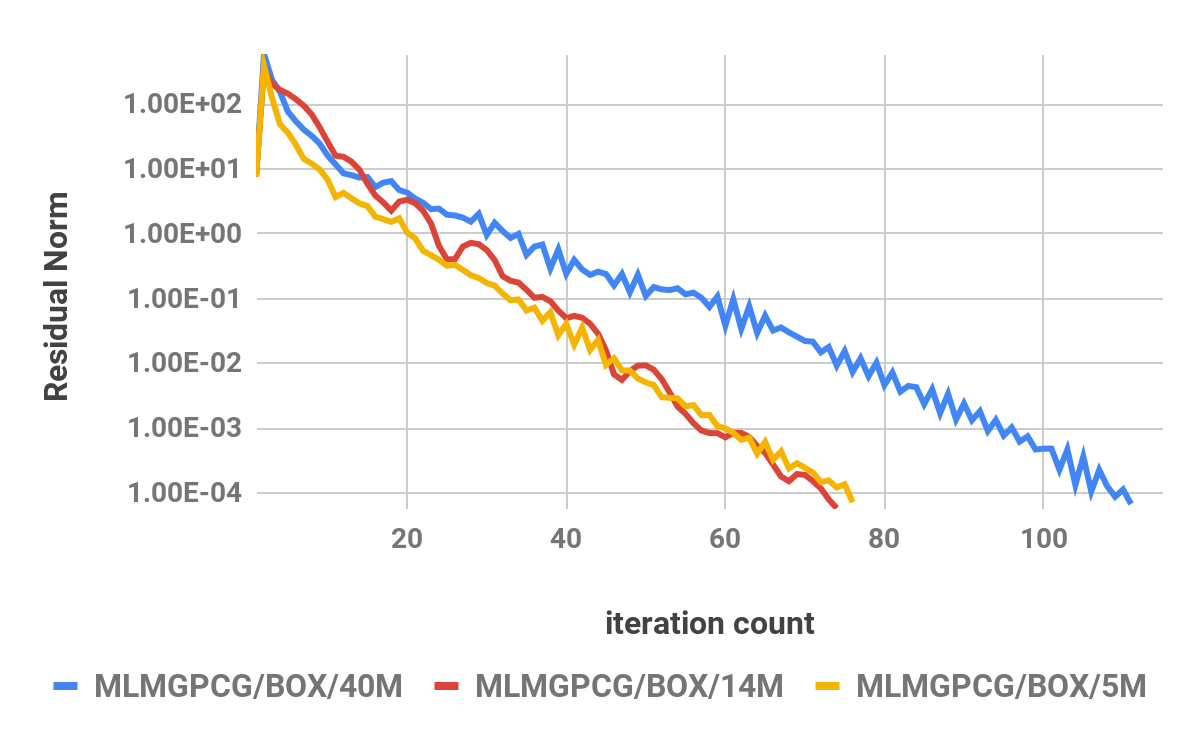
\includegraphics[width=\textwidth]{BBMG/MLMGPCG_BOX.png}
 \end{subfigure}	
  \begin{subfigure}[t]{0.5\textwidth}
 \centering
 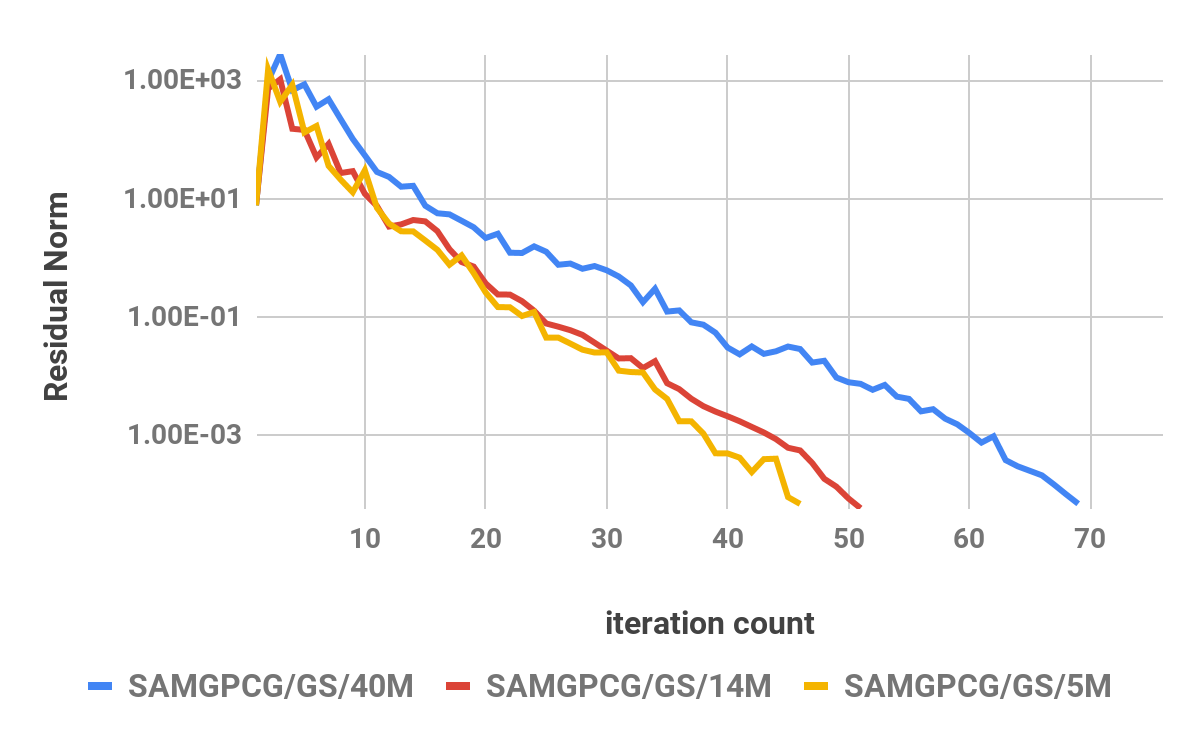
\includegraphics[width=\textwidth]{BBMG/SAMGPCG_GS.png}
 \end{subfigure}
 \begin{subfigure}[t]{0.5\textwidth}
 \centering
 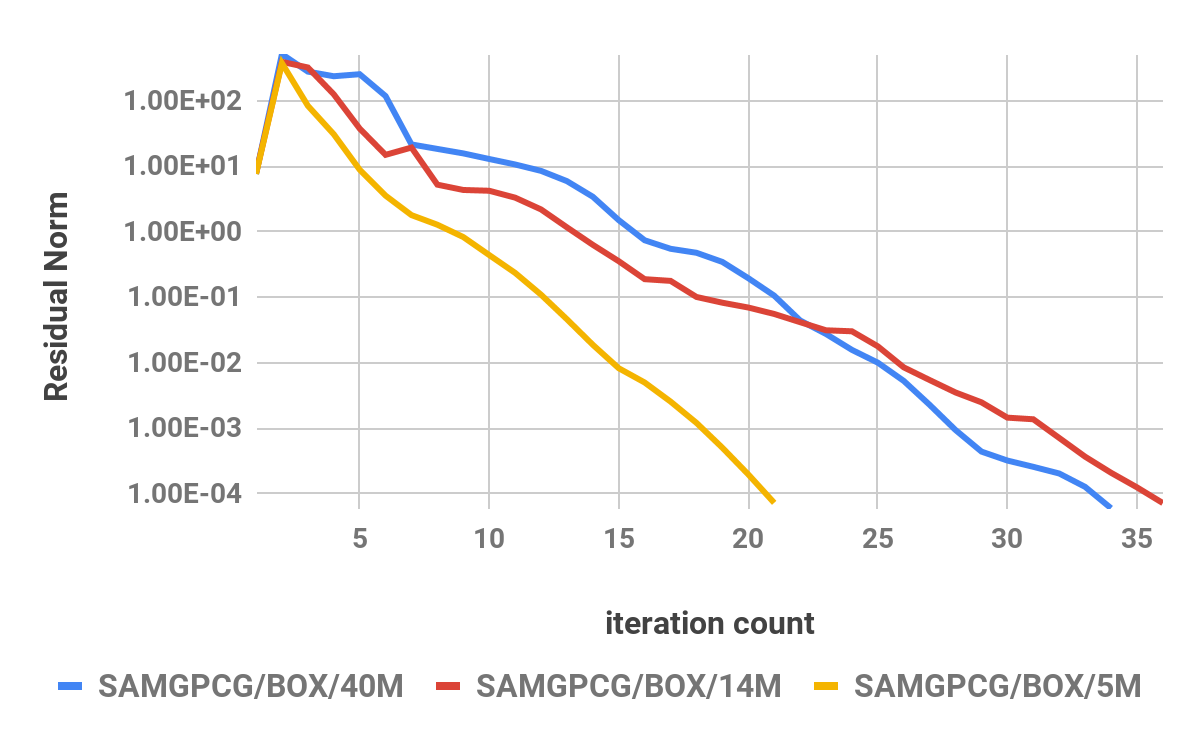
\includegraphics[width=\textwidth]{BBMG/SAMGPCG_BOX.png}
 \end{subfigure}	
\caption{Convergence plot for the bird beak example. In all cases multigrid hierarchy contains 4 levels, and 3-1-3 smoothing iterations were applied. Top left: MLMGPCG with Gauss-Seidel smoother with 40M/14M/5M active voxels.Top right: MLMGPCG with box smoother with 40M/14M/5M active voxels.Top left: SAMGPCG with Gauss-Seidel smoother with 40M/14M/5M active voxels.Top right: SAMGPCG with box smoother with 40M/14M/5M active voxels.}
\label{fig:Bird_Beak_Convergence_Test}
\end{figure}